% Work in progress, not final

\chapter{Self-sovereign Identity}\label{chapter: ssi}

Health care, social security, education, access to financial services — this is just a small list of requirements that are essential for a decent life and are usually taken for granted by people in the Western world. Yet there are more than 1.1 billion people worldwide who cannot provide identification and thus cannot access the most basic services. Digital identities could make a significant contribution towards solving this problem and give people the chance to participate in society on a more equal playing field. \cite{world_bank_11_2017}

As already mentioned in chapter \ref{chapter: Introduction}, however, current implementations of such digital identities are insufficient for the problems of our modern times. \cite{soltani_survey_2021} divided these problems into four categories:
\begin{enumerate}
	\item Data Ownership and Governance
	\item Password-Based Authentication
	\item Fragmented Identity Data
	\item Data Breaches and Identity Fraud
\end{enumerate}
The former describes the fact that users have no ownership over their digital identities and thus cannot exercise any control over them. Service providers often take advantage of this and use collected data to create comprehensive profiles of their users and thus sell tailored advertising space on corresponding marketplaces for high figures. The lack of control also means that service providers can temporarily or permanently deny users access to their digital identity at any time. At the beginning of 2021, this led to much discussion as the account of former U.S. President Donald Trump was permanently banned from Twitter. One of the central concerns was whether service providers have too much power over users' liberties \cite{noor_should_2021}. In addition, given the frequent and often repeated use of weak passwords, the heavy reliance on password-based authentication is a security risk that may lead to identity theft. If a user wants to be as secure as possible, they need to use different and as complex as possible passwords for each of their accounts, which quickly becomes a complex undertaking without a password manager. A study by the password manager LastPass, for example, found that a business customer manages an average of 191 passwords \cite{steel_lastpass_2017}. While the use of such tools greatly simplifies the management of passwords, they too can pose a major security risk and do not completely protect the user \cite{oesch_that_2020, ormandy_password_2021, toth_you_2021}. Alternatives such as single sign-on, where users authenticate to other service providers using for example their Google account, can solve this problem but lead to even greater dependency and centralization. The third issue involves identity data being spread across a large set of service providers, making it difficult to maintain. As a result, duplicates, errors, and outdated data sets are common. The lack of open standards also complicates interoperability between providers, which could theoretically be used to retrieve, move, or delete data. \cite[pp. 2-3]{soltani_survey_2021}
One of the biggest problems, however, are data breaches. In June 2021 alone, there were 235 breaches with 1.16 billion stolen records, with a total of 18.9 billion records stolen in 1,785 breaches in the first half of 2021 \cite{risk_based_security_data_2021}. Looking at the past, there have been quite a few major hacks \cite{swinhoe_15_2021}, including: 

\begin{itemize}
    \item Yahoo (2013): 3 billion accounts
    \item Alibaba (2019): 1.1 billion entries
    \item LinkedIn (2021): 700 million accounts
    \item Marriott (2018): 500 million customer records
\end{itemize}

A survey of 413 people by \cite{mayer_now_2021} found that 73 \% of participants had been affected by at least one but an average of 5.3 data breaches. In addition, the majority blamed themselves for the breaches, with only 14 \% aware that service providers were responsible.

Kim Cameron, who worked at Microsoft from 1999 to 2019 most recently as Chief Architect of Identity, recognized these problems as early as 2005 in a blog post \cite{cameron_laws_2005}:

\begin{displayquote}
    \textit{"The Internet was built without a way to know who and what you are connecting to. This limits what we can do with it and exposes us to growing dangers. If we do nothing, we will face rapidly proliferating episodes of theft and deception that will cumulatively erode public trust in the Internet."}
\end{displayquote}

Among other things, he discusses the causes and effects of a missing identity layer on the Internet and defines ten laws of identity. These in combination with the emergence of blockchain technology and various new standards led to the increasingly popular concept of \acf{SSI} in recent years. It is intended to eliminate the shortcomings of today's established concepts by placing the user in the center and giving them back complete control over their identity data. The user can decide what, to whom and how much data is shared without being dependent on a central authority. [\citealp[pp. 6-7]{struker_grundlagen_2021}; \citealp[pp. 8-9]{tobin_inevitable_2017}]

\ac{SSI} is a completely new approach to digital identities on the Internet and is seen as a paradigm shift that deeply affects the infrastructure and power distribution of the Internet \cite[p. 3]{reed_decentralized_2021}. For a deeper look at the topic, this chapter takes a closer look at Self-sovereign Identity. For this purpose, the concept of identity and the different types of identities will be discussed first. This is followed by a historical look at the different stages of digital identities, taking a closer look at the previous concepts of \ac{SSI}. After a basic foundation has been built, standards that have been established in recent years and are intended to make \ac{SSI} feasible in reality are described. Finally, the \ac{SSI} architecture with its components and roles will be looked at.

% Next: Maybe add a short Intro like i did in chapter 1. --> Definition, Motivation, Problem Definition, Vision

    \section{Identity}

    What defines a human being? One would probably get various answers to this question, such as its name, gender, place of residence, profession, hobbies, religion, charitable activities, party affiliation or even a combination of all these characteristics. The concept of identity combines all of these personal characteristics into one term that can define a person. \cite[p. 206]{claus_identity_2001} describes in his work that a person's identity is not just a single, fixed construct, but consists of several partial identities. Thus, depending on the context in which a person finds itself, it takes on one of its various partial identities, which represents it as a human being more or less. For example, a partial identity for health care consists of medical history while the partial identity towards work contains certificates. Nevertheless, these different parts of the identity are not necessarily considered separately, as they can also overlap in certain aspects of information. It is important to mention that a person decides which information to share at which time towards which entity. In \ref{figure: alice} the concept of partial identities is illustrated exemplarily by a person Alice.
    
    \begin{figure}[ht]
        \centering
        \makebox[\textwidth]{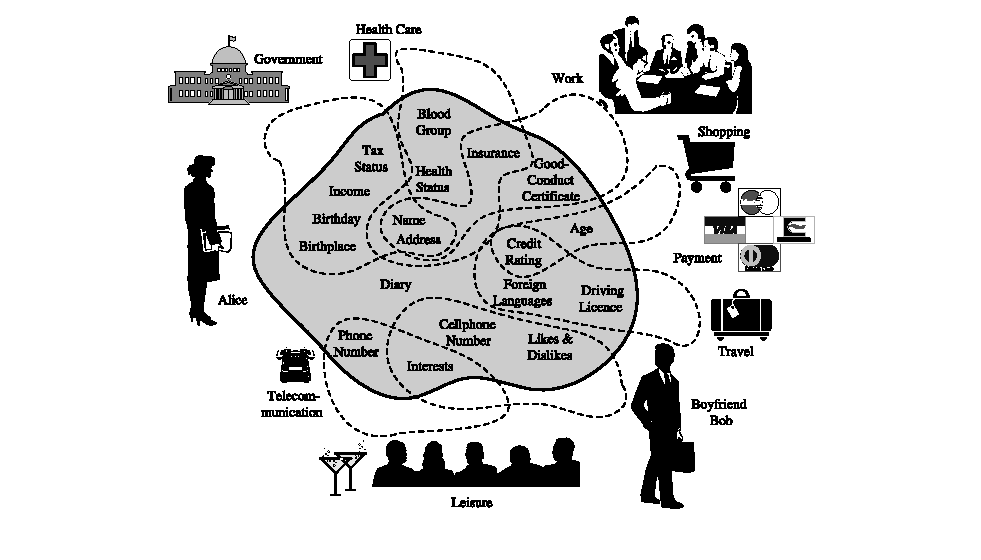
\includegraphics[width=\textwidth]{img/2_alice.eps}}
        \caption{Partial Identities of Alice extracted from \cite{claus_identity_2001}}
        \label{figure: alice}
    \end{figure}

    An important balancing act is to disclose the right amount of data in order to maintain anonymity, but also to provide the other person with the necessary information. For the purchase of a water, the kiosk vendor should not ask for any personal data, whereas verification of age when buying alcohol is also necessary from a purely legal point of view. In reality, official documents, such as state identification documents, or sometimes unofficial documents, such as customer cards, are usually used for such proof of identity. Here, users have full control over their documents as they are under their control, and only they can decide self-sovereignly whom and when to show them. Official identification documents are also produced and standardized to ensure the highest possible level of security and interoperability.Other countries can verify such documents without explicitly contacting authorities, but simply by looking at the document.  Confidence in the validity of the data arises from the fact that the verifying party trusts the authority issuing the document. \cite[p. 6]{struker_grundlagen_2021}

    As a result of the increasing digitalization of various branches of life, many processes are shifting to the digital world. Digital identities, which are similar to analog identities in terms of their basic idea, are now being used for interacting with digital services. They allow entities, such as people or objects, to authenticate themselves online through certain attributes and thus prove their identity [\citealp[p. 103]{meinel_blockchain_2020}; \citealp{bundesdruckerei_so_2020}]. Unlike analog identities, these analog documents cannot be used easily in the digital world. Digital identities have diverged in their characteristics from the original analog identities. [\citealp[p. 10]{struker_grundlagen_2021}; \citealp[p. 2]{ehrlich_self-sovereign_2021}] 
    
    // TODO: Incorporate Cameron, Online funktion ausweis eID
        
	\section{Stages}
	% Four phases @Allen, add problems of those; types of identities, comparison
	\section{Standards}
	    \subsection{Overview}
	    \subsection{Decentralized Identifier}
	    % Zookos Triangle, Standard definition, did methods, did doc, lifecycle
	    \subsection{Verifiable Credentials}
	    % Lifecycles, 
		\subsection{DIDComm}
		\subsection{Zero Knowledge Proofs}
	\section{Architecture}
	\subsection{Roles}
	\subsection{Components}